\documentclass[a4paper, 11pt]{report}
\usepackage{epsfig}
\usepackage{graphics}
\usepackage{multirow}
\usepackage{multicol}
\usepackage{fancyhdr}
\usepackage{lastpage}
\usepackage{latexsym}
\usepackage[hang, scriptsize, bf]{caption}

\usepackage[utf8]{inputenc}

\usepackage{enumerate}

\usepackage{tikz}
\usepackage[european]{circuitikz}

\usepackage{stackengine}
\usepackage{scalerel}
\usepackage{xcolor}

\usepackage{tikz-qtree}
\usetikzlibrary{arrows,shapes,snakes,positioning,automata}
\usetikzlibrary{shapes.multipart}
\usetikzlibrary{patterns,shapes}


\usepackage{wasysym}

\usepackage{algorithmic}
\usepackage{listings}

\usepackage{multirow}
\usepackage{multicol}

\usepackage{hhline}
\usepackage{array}
\usepackage{longtable}


\renewcommand{\figurename}{Obrázek}

\newcommand\dangersign[1][2ex]{%
  \renewcommand\stacktype{L}%
  \scaleto{\stackon[1.3pt]{\color{red}$\triangle$}{\tiny\bfseries !}}{#1}%
}
%-------------------------------------------------------------------------------

\textwidth      170mm
\textheight     240mm
\hoffset        -10mm 
\voffset        -10mm
\oddsidemargin   5mm
\evensidemargin -5mm
\topmargin	    -5mm

%-------------------------------------------------------------------------------

\newcommand{\eduTitle}{Zadání laboratoře}
\newcommand{\eduID}{3}
\newcommand{\eduTopic}{VA charakteristika a pracovní bod součástky}
\newcommand{\eduDetails}{
\footnotesize
Cíle: Odměřit Volt-Ampérovou (VA) charakteristiku součástky a 
určit pracovní bod součástky v obvodu.
}
%
\newcommand{\subjIDlong}{Elektronika pro informační technologie}
\newcommand{\schoolDlong}{Vysoké učení technické v Brně}
\newcommand{\schoolDshort}{VUT v Brně}
\newcommand{\facultylDlong}{Fakulta informačních technologií}
\newcommand{\facultylDshort}{FIT}
%
\newcommand{\subjIDshort}{IEL}
%
\newcommand{\actYear}{2024}
\newcommand{\acadYear}{2024/2025}

\usepackage[hidelinks]{hyperref}

%-------------------------------------------------------------------------------

\newcommand*\circled[1]{\tikz[baseline=(char.base)]{
            \node[shape=circle,draw,inner sep=2pt] (char) {#1};}}

%-------------------------------------------------------------------------------

\newcounter{cntInfo}
\newcommand{\info}[3]{\refstepcounter{cntInfo}
\paragraph*{
\circled{\thecntInfo}~{\sc \fbox{#1}} {\sc #2}  
} 
\paragraph{\textmd{#3}} }

%-------------------------------------------------------------------------------

\begin{document}

%-------------------------------------------------------------------------------

\pagestyle{fancy}
\renewcommand{\headrulewidth}{0pt}
\renewcommand{\theenumi}{\Alph{enumi}}  
\lhead{}
\chead{}
\rhead{}
\lfoot{\centering
\tiny \itshape \eduTitle ~č. \eduID \hspace{0.1mm} z předmětu \subjIDshort \hspace{1mm} 
(ak. r. \acadYear). \copyright~\actYear~Josef~Strnadel,~\facultylDshort~\schoolDshort. Připomínky zasílejte na \href{mailto:strnadel@fit.vut.cz}{strnadel@fit.vut.cz}\\ 
Časové razítko PDF dokumentu [\pdfcreationdate]. 
Sazba byla provedena systémem \LaTeX.
 }
\cfoot{}
%-------------------------------------------------------------------------------

%-------------------------------------------------------------------------------

\begin{center}
\scalebox{0.1}{
\includegraphics{FIT_cernobile_CZ.pdf}}
\parbox{120mm}{
\textsc{\footnotesize\schoolDlong}, 
\textsc{\footnotesize\facultylDlong}\\
}
{
\Large
\textsc{\subjIDlong} (\textsc{\subjIDshort}), \textsc{ak. r. \acadYear}}

\hrulefill

\vspace{4mm}
\parbox{\linewidth}{
\centering
%
{\Huge \textsc{\eduTitle~č.~\fbox{\eduID}}}\\
{\textsc{,,\eduTopic''}}\\

}

\end{center}

{\it \eduDetails}

\hrulefill

%-------------------------------------------------------------------------------
\info{Motivace}{aneb ,,Proč tomu věnovat čas a jaké kompetence lze získat ?''}{
Na základně experimentů budete schopni stanovit 
VA charakteristiku 
součástek, porozumět jejímu významu a prakticky využít VA charakteristiku k určení pracovního bodu součástky v obvodu.
%
\\[4mm]
Zapamatujte si:
}

\vspace{-2mm}
\begin{itemize}
\item
\textsc{VA charakteristika} součástky vyjadřuje 
závislost (vztah) mezi 
napětím na součástce 
a 
proudem procházejícím součástkou;
tato závislost může být lineární, ale také nelineární.
\vspace{-2mm}
\item
\textsc{Pracovní bod} součástky 
je bodem VA charakteristiky, 
který odpovídá pracovním podmínkám součástky (proud, napětí) v konkrétním obvodu\footnote{potřebné pracovní
podmínky lze zajistit 
např. 
omezením proudu procházejícího součástkou pomocí rezistoru zapojeného v sérii s ní}.
\end{itemize}

%-------------------------------------------------------------------------------
\info{Výstup a způsob jeho hodnocení}{aneb ,,Co se ode mne očekává a co za to ?''}{
Za i) provedení měření nezbytných pro stanovení VA charakteristiky součástek, 
záznam výsledků měření formou tabulky,
ii) vynesení závislostí naměřených hodnot do grafu 
a iii) grafické stanovení pracovního bodu zadané součástky v obvodu lze získat až {\bf 3 body}.
}

%-------------------------------------------------------------------------------
\info{Prostředky}{aneb ,,Co je k dispozici ?''}{
~
}

Zdroj ss. napětí s omezením proudu,
nepájivé pole, 
krabička s prvky pro konstrukci obvodů (propojovací vodiče, součástky -- 
potenciometr pro regulaci hodnoty  napětí,
rezistor pro omezení proudu obvodem, 
nelineární součástka),
měřicí přístroje (2x multimetr). 
\\

%-------------------------------------------------------------------------------
\info{Základní schéma(ta)}{aneb ,,Z čeho se bude vycházet ?''}{
~
}

\vspace{-6mm}
\begin{figure}[h!]
  \begin{center}


\scalebox{0.95}{
    \begin{circuitikz}
      \draw (0,0)
      to[american voltage source,invert,v<=5~V] (0,2) % The voltage source
      to[short] (1.25,2)
      to[vR, mirror] (1.25,0)
      to[short] (0,0)
    ;
    
    \node at(1.75,1.75) {$R_{pot}$};

    \draw(1.725,1.275)
      to[short] (2.0,1.275) node (out1) [ocirc] {}  node[right] {\scriptsize 1}
      ;

   \draw(1.25,0) node[circ] {}
      to[short] (2.0,0) node (out2) [ocirc] {}  node[above left] {\scriptsize 2}
   ;
    
    \node (out22) at (2,0.1) {};

\draw (out22) to[open, v<={\hspace{0mm}$U_0$}] (out1);
    
     \draw(-1,-.25) node {\scriptsize a)};
     \draw(2,-1.25) node {~};
    \end{circuitikz}
    }
 \scalebox{.90}{
    \begin{circuitikz}
      \draw (1,2) node (in1) [ocirc]{} node[above] {\scriptsize 1}
     to[R,  l_=$R_S$, i_=$I$] (4,2)
      to[thR, invert, l_=$R_N$, i_=$I_N$] (4,0) % The resistor
      to[short] (1,0)
      to[short] (1,0) node (in2) [ocirc]{}  node[above right] {\scriptsize 2};
\draw (in1) to[open, v>=$U_0$] (in2);

\draw node (A) at (4.5,0) {}
node (B) at (4.5,2) {}
(B) to[open, v^=$U_{N}$] (A);
\draw node (C) at (1.5,2.25) {}
node (D) at (3.5,2.25) {}
(C) to[open, v^=$U_{S}$] (D);
     \draw(0.5,0) node {\scriptsize b)};
     \draw(2,-1.0) node {~};

    \end{circuitikz}

} 
\hspace{0mm}
%
\scalebox{.90}{
    \begin{circuitikz}
      \draw (1,2) node (in1) [ocirc]{}  node[above] {\scriptsize 1}
     to[R,  l_=$R_S$, i_=$I$] (4,2)
      to[thR, invert, l_=$R_N$, i_=$I_N$] (4,0) % The resistor
      to[ammeter, mirror, color=red] (1,0)
      to[short] (1,0) node (in2) [ocirc]{}  node[above right] {\scriptsize 2}
%
(B) to[open, v^=$U_{N}$] (A);
\draw node (C) at (1.5,2.25) {}
node (D) at (3.5,2.25) {}
(C) to[open, v^=$U_{S}$] (D);
      \draw[color=red] (4,2)
      to[short, *-] (6.5,2)
      to[voltmeter] (6.5,0)
      to[short, -*] (4,0)
      ;
\draw (in1) to[open, v>=$U_0$] (in2);


     \draw(0.5,0) node {\scriptsize c)};
     \draw(1,-1.0) node {};
    \end{circuitikz}

}


\vspace{-8mm}
   \caption{a) obvod pro regulaci velikosti napětí $U$ pomocí potenciometru $R_{pot}$; obvod s lineární součástkou (rezistor, $R_S$) a nelineární součástkou (dioda, $R_N$): b) základní schéma a veličiny, c) rozšíření o měřicí přístroje. 
}
   \label{fig_nonlinear1}
  \end{center}
\vspace{-4mm}
\end{figure}


%-------------------------------------------------------------------------------
\info{Postup samostatných činností}{aneb ,,Co dělat a na co si dát pozor ?''}{
~
}

\vspace{-8mm}

\begin{enumerate}[\bf {Experiment} 1:]

\item

V nepájivém poli zapojte obvod dle Obr. \ref{fig_nonlinear1}a\footnote{pozn.: 
potenciometr $R_{pot}$ má tři vývody: 
dva vývody z krajů odporové dráhy,
třetí vývod z kontaktu pohyblivého po odporové dráze (tzv. jezdec) např. s pomocí otočného knoflíku či táhla},
poté
k obvodu připojte voltmetr\footnote{multimetr v režimu voltmetru} tak, aby jím bylo možné měřit napětí $U_0$;
otáčejte knoflíkem potenciometru a
sledujte vliv polohy knoflíku na $U_0$. Obvod nerozpojujte -- využijete jej při dalším experimentu.

\item

\begin{enumerate}[i)]
\item 
Zapojte obvod dle Obr. \ref{fig_nonlinear1}b
a rozšiřte jej dle Obr. \ref{fig_nonlinear1}c.
Spojením obvodů~z~Obr.~\ref{fig_nonlinear1}a,c vytvořte obvod pro odměření VA charakteristiky
nelineární součástky $R_N$\footnote{přemístěním voltmetru lze  odměřit také VA charakteristiku 
lineární součástky $R_S$, popř. sériového zapojení $R_S$, $R_N$}.
\item 
Pomocí potenciometru krokujte hodnotu $U_0$ (viz např. tab. níže).
Pro každou hodnotu $U_0$ 
do tabulky zapište a poté do grafu vyneste závislost mezi $U_N$ a $I_N$.
\end{enumerate}

\vspace{-2mm}
\begin{table}[h]
\hspace{35mm}
\scalebox{0.7}{
\begin{tabular}{|c||c|c|c|c|c|c|c|c|c|c|}
\hline
\bf $U_0$ 
&\parbox{8mm}{\centering 0}
&\parbox{8mm}{\centering 0,1}
&\parbox{8mm}{\centering 0,2}
&\parbox{8mm}{\centering 0,4}
&\parbox{8mm}{\centering 0,6}
&\parbox{8mm}{\centering 0,8}
&\parbox{8mm}{\centering 1}
&\parbox{8mm}{\centering 3}
&\parbox{8mm}{\centering 5}&\multirow{2}{*}{[V]}\\
\cline{1-10}
\bf $U_N$ &&&&&&&&&&\\
\hline
\bf $I_N$ &&&&&&&&&&[$\mu$A]\\
\hline
\end{tabular}
}
\label{tab:va}
\end{table}
\vspace{-2mm}

\item

\begin{enumerate}[i)]
\item
Pro vyučujícím zadanou hodnotu $U_0$
určete pracovní bod $P_N$ nelineární součástky $R_N$ v~obvodu z Obr. \ref{fig_nonlinear1}b,c;
 při určení postupujte dle ii) a/nebo iii) níže.

\item
Odměřte závislost napětí $U_S + U_N$ 
na $I_N$
(tj., VA charakteristiku série $R_S + R_N$).
Z $U_0$ na ose $U$ vztyčte kolmici; 
jejím průnikem s VA charakteristikou pro $R_S + R_N$
je bod $P_{SN}$. Z $P_{SN}$ veďte rovnoběžku s osou $U$
a vyznačte její průnik s osou $I$ (bod $I_P$)
a s VA charakteristikou pro $R_N$ (bod $P_N$),
odečtěte $U_P$.

\item
Vypočítejte či odměřte hodnotu proudu nakrátko ($I_K$) zdroje $U_0$ s vnitřním odporem $R_S$\footnote{proud 
při nahrazení $R_N$ z Obr. \ref{fig_nonlinear1}b,c vodičem; $I_K = U_0 / R_S$}.
Bod $P_N$ je průnik úsečky $I_K$$U_0$ a VA charakteristiky pro $R_N$. 

\end{enumerate}



\end{enumerate}

\begin{figure}[h]
\vspace{-5mm}
\centering
\footnotesize

\parbox{20mm}{
~
}
\parbox{2mm}{
\centering
\vspace{-4mm}
a)
}
\hspace{-8mm}
\scalebox{.9}{
\hspace{1.5mm}
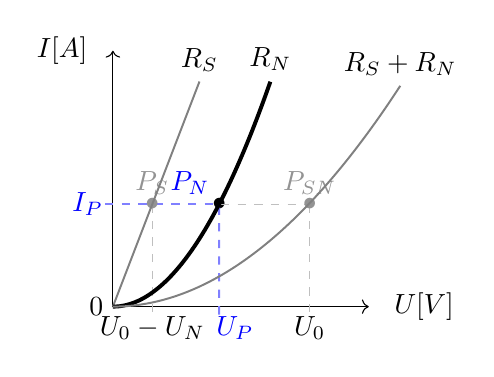
\begin{tikzpicture}
\draw[->] (0,0) -- (0,3.25) node[left=2mm] {$I [A]$};
\draw[->] (0,0) -- (3.25,0) node[right=2mm] {$U [V]$};

% prac. bod
\node[inner sep=-4pt]  (n0) at (1.35,1.3) {$\bullet$};
\node[above left] at (n0) {\textcolor{blue}{$P_N$}};
\node[left] at (0,1.3) {\textcolor{blue}{$I_P$}};
\node[below] at (1.55,0) {\textcolor{blue}{$U_{P}$}};

% ... horiz (P)
\draw[line width=.25mm, dashed, color=blue!50] (-.1,1.3) -- (n0);
% ... vert. (P)
\draw[line width=.25mm, dashed, color=blue!50] (1.35, -.1) -- (n0);


% ... horiz P -> (S+N)
\draw[line width=.1mm, dashed, color=gray!50] (n0) -- (2.5,1.3);
% ... vert. (S+N)
\draw[line width=.1mm, dashed, color=gray!50, text=gray!85] (2.5,1.3) node[above] {$P_{SN}$} node{$\bullet$} -- (2.5,-.1);

% ... vert. (S)
\draw[line width=.1mm, dashed, color=gray!50, text=gray!85] (0.5,1.3) node[above] {$P_S$} node{$\bullet$} -- (0.5,-.1);


% zatez. prim.
\node[inner sep=-4pt] (npx) at (0.0, 2.85) {};
\node[inner sep=-4pt] (npy) at (2.5, 0.0) {};
\node[below] at (npy) {$U_0$};
\node[below] at (0.5,0) {$U_0 - U_N$};

\draw[scale=1.0,domain=0.0:1.1,smooth,variable=\x,gray, line width=.25mm]  plot ({\x},{\x*2.6})  node[above=0mm] {\textcolor{black}{$R_S$}};
\draw[scale=1.0,domain=0.0:2.0,smooth,variable=\x,black, line width=.5mm]  plot ({\x},{\x*\x/1.4})  node[above=0mm] 
{\textcolor{black}{$R_N$}};
\draw[scale=1.0,domain=0.0:3.65,smooth,variable=\x,gray, line width=.25mm]  plot ({\x},{\x*\x/4.75}) node[above=0mm] {\textcolor{black}{$R_S + R_N$}};

\node[left] at(0,0) {0};

\end{tikzpicture}
}
%
%
\hspace{12mm}
\parbox{2mm}{
\centering
\vspace{-4mm}
b)
}
\hspace{-8mm}
%
%
\scalebox{.9}{
\hspace{1.5mm}
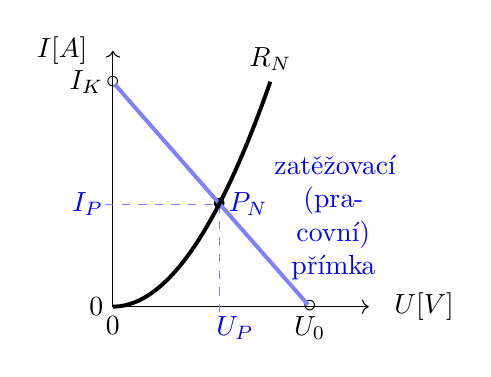
\begin{tikzpicture}
\draw[->] (0,0) -- (0,3.25) node[left=2mm] {$I [A]$};
\draw[->] (0,0) -- (3.25,0) node[right=2mm] {$U [V]$};

% prac. bod
\node[inner sep=-4pt]  (n0) at (1.35,1.3) {$\bullet$};
\node[right] at (n0) {\textcolor{blue}{$P_N$}};
\node[left] at (0,1.3) {\textcolor{blue}{$I_P$}};
\node[below] at (1.55,0) {\textcolor{blue}{$U_{P}$}};

%% ... horiz (P)
\draw[line width=.1mm, dashed, color=blue!50] (-.1,1.3) -- (n0);
% ... vert. (P)
\draw[line width=.1mm, dashed, color=blue!50] (1.35,1.3) -- (1.35,-.1);

% zatez. prim.
\node[inner sep=-4pt] (npx) at (0.0, 2.85) {$\circ$};
\node[inner sep=-4pt] (npy) at (2.5, 0.0) {$\circ$};
\draw[line width=.5mm, solid, color=blue!50] (npx) -- (npy)    node[above=2mm] {\hspace{6mm}\parbox{15mm}{
\centering
\textcolor{blue}{zatěžovací (pracovní) přímka}}};
\node[left] at (npx) {$I_{K}$};
\node[below] at (npy) {$U_0$};

\draw[scale=1.0,domain=0.0:2.0,smooth,variable=\x,black, line width=.5mm]  plot ({\x},{\x*\x/1.4})  node[above=0mm] 
{\textcolor{black}{$R_N$}};

\node[left] at(0,0) {0};
\node[below] at(0,0) {0};

\end{tikzpicture}
}

\vspace{-2mm}
\caption{Ilustrace k pracovnímu bodu nelineární součástky z Obr. \ref{fig_nonlinear1}b,c:
$U_0$~--~napětí naprázdno napájecího zdroje,
$I_K$~--~proud nakrátko zdroje $U_0$ s vnitřním odporem $R_S$,
$P_N$~--~pracovní bod nelineární součástky $R_N$, 
$P_S$~--~p.b. lineární součástky $R_S$,
$P_{SN}$~--~p.b. série $R_S$, $R_N$ (napájecího zdroje);
$I_P$~--~proud procházející součástkami $R_S$ a $R_N$,
$U_P = U_N$~--~napětí na nelineární součástce $R_N$ v~pracovním bodě $P_N$;
$(U_0 - U_N)$~--~napětí na lineární součástce $R_S$ v prac. bodě $P_S$.
}
\label{fig:pracovni_bod}
\vspace{-0mm}
\end{figure}


%-------------------------------------------------------------------------------
\vspace{-5mm}
\info{Shrnutí, vyhodnocení a interpretace výsledků}{aneb ,,Jaká jsou zjištění ?''}{
Experimentálně jste mohli ověřit, že i) ne každá součástka má lineární VA charakteristiku
a ii) stav každé součástky je, v daném čase, dán jejím pracovním bodem.
Špatně nastavený pracovní bod  může způsobit nevratné poškození součástky (např. průraz svítivé diody) a následné selhání služeb (např. signalizace stavu) poskytovaných nadřazeným systémem.
}

%-------------------------------------------------------------------------------
\info{K zamyšlení/zapamatování}{aneb ,,Něco do dalšího studia a života.''}{
V praxi lze znalost 
tvaru VA charakteristiky, 
hodnoty $U_0$ 
a 
požadovaného pracovního bodu ($P_N$) nelineární součástky ($R_N$)
využít 
např. 
ke stanovení hodnoty odporu rezistoru $R_S$ zapojeného v sérii s $R_N$. 
Průnikem přímky $U_0$$P_N$ s osou $I$ vznikne bod $I_K$ (viz Obr. \ref{fig:pracovni_bod}b); 
$R_S = U_0 / I_K$. 
Alternativně (viz Obr. \ref{fig:pracovni_bod}a): $R_S$ = $U_S / I_S$ = $(U_0 - U_N) / I_P$.
}


\end{document}
